%=====================================================================================
%& -job-name=erc20-multiple-withdrawal-attack
\documentclass[compsoc, conference, letterpaper, 10pt, times]{IEEEtran}

% !TEX root = ../main.tex

%------------------------IEEE----------------------%

% = = = IEEE Recommended
\usepackage{mdwmath}
\usepackage{mdwtab}
\usepackage{eqparbox}

% = = = IEEE Recommended (Double-column)
\usepackage{fixltx2e}
\usepackage{stfloats}

% = = = Compact Bibliography
\usepackage{bibspacing}
\setlength{\bibspacing}{\baselineskip}
%\usepackage{authblk}
% NOTE: IEEE does not allow algorithm2e



%------------------------Packages----------------------%

% = = = Graphics
\usepackage[pdftex]{graphicx}
\graphicspath{{figures/}}
\DeclareGraphicsExtensions{.jpg,.png}

% = = = Subfig (note not subfigure)
\usepackage[caption=false,font=footnotesize]{subfig}

% = = = Math Symbols
\usepackage{amsmath}
%\usepackage{amstext,amssymb,amsthm}
\usepackage{bbm}
\usepackage{stmaryrd}

% = = = Other
\usepackage{array}
\usepackage{color}
\usepackage[hyphens]{url}
\usepackage[pdftitle=Title,pdfauthor=Anonymous]{hyperref}
\usepackage{xcolor}

% = = = Listings
\usepackage{listings}

% Enable syntax highlighting
\lstset {
    tabsize=4,
    language=c++,
    basicstyle=\scriptsize,
    upquote=true,
    %aboveskip={1.5\baselineskip},
    %belowskip={1.5\baselineskip},
    columns=fixed,
    showstringspaces=false,
    extendedchars=true,
    numbers=left,
    stepnumber=1,
    breaklines=true,
    prebreak=\raisebox{0ex}[0ex][0ex]{\ensuremath{\hookleftarrow}},
    showtabs=false,
    showspaces=false,
    showstringspaces=false,
    identifierstyle=\ttfamily,
    keywordstyle=\color[rgb]{0,0,1},
    commentstyle=\color[rgb]{0.133,0.545,0.133},
    stringstyle=\color[rgb]{0.627,0.126,0.941},
}

\lstdefinestyle{interfaces}{
  float=t,
  floatplacement=t}

%------------------------END----------------------%  
  


% !TEX root = ../main.tex
%------------------------Custom Commands----------------------%

% = = = Latin Short-forms (ie, eg, etc, et al)
\usepackage{xspace}
\newcommand{\etal}{\textit{et al.}\xspace}
\newcommand{\etc}{\textit{etc.}\xspace}
\newcommand{\ie}{\textit{i.e.,}\xspace}
\newcommand{\eg}{\textit{e.g.,}\xspace}
\newcommand{\cf}{\textit{cf.}\xspace}
\newcommand{\supra}{\textit{Supra}\xspace}

% = = = Arrow -> (\lt)
\newcommand{\lt}{$\rightarrow$\xspace}

% = = = Keywords (kw)
\newcommand{\kw}[1]{\textsf{#1}}

% = = = Colored text (textblue)
\newcommand{\textblue}[1]{\textcolor{blue}{#1}}

% = = = Compact Lists (compactlist, compactlistn)
\newenvironment{compactlist}
  {\begin{itemize} 
  \setlength{\itemsep}{0pt} 
  \setlength{\parskip}{0pt}} 
  {\end{itemize}}
  
\newenvironment{compactlistn}
  {\begin{enumerate} 
  \setlength{\itemsep}{0pt} 
  \setlength{\parskip}{0pt}} 
  {\end{enumerate}}
  
\renewcommand{\labelitemi}{$\bullet$}
  

%------------------------Crypto----------------------%  

% = = = Zp, Gq and Zq
\newcommand{\Zp}{\mathbb{Z}^{*}_{p}}
\newcommand{\Zq}{\mathbb{Z}_{q}}
\newcommand{\Gq}{\mathbb{G}_{q}}

% = = = Encryption, etc.
\newcommand{\Enc}[1]{\mathsf{Enc}(#1)}
\newcommand{\EncB}[1]{\llbracket #1 \rrbracket}
\newcommand{\ReRand}[1]{\mathsf{ReRand}(#1)}
\newcommand{\Hash}[1]{\mathcal{H}(#1)}
\newcommand{\Sign}[1]{\mathsf{Sig}(#1)}
\newcommand{\Comm}[1]{\mathsf{Comm}(#1)}
\newcommand{\Open}[1]{\mathsf{Open}(#1)}

% = = = Tuples
\newcommand{\tuple}[1]{\left \langle #1 \right \rangle}


%-------------------Custom for Paper----------------------%

% = = = Name
\newcommand{\Name}{\textsf{System Name}\xspace}
\newcommand{\dapp}{DApp\xspace}
\newcommand{\dapps}{DApps\xspace}









\IEEEoverridecommandlockouts
\IEEEpubid{\makebox[\columnwidth]{} \hspace{\columnsep}\makebox[\columnwidth]{ }}

%\usepackage[short,nodayofweek]{datetime}
%\usepackage[noadjust]{cite}
%\usepackage{graphicx}
%\usepackage[T1]{fontenc}
%%footnote
%\usepackage[flushmargin]{footmisc}
%\addtolength{\footnotesep}{1mm}
%\renewcommand{\thefootnote}{\textbf{\arabic{footnote}}}
%%enumeration
%\usepackage{float}
%\usepackage[none]{hyphenat}
%\usepackage{enumitem}
%\setlist[enumerate]{label=\arabic*-,leftmargin=*,align=left}
%%watermark
%\usepackage{draftwatermark}
%\SetWatermarkText{Draft: \today}
%\SetWatermarkColor[gray]{0.7}
%\SetWatermarkFontSize{0.5cm}
%\SetWatermarkAngle{90}
%\SetWatermarkHorCenter{1cm}
%%footer
%\usepackage{lastpage}
%\usepackage{fancyhdr}
%\fancyhead{}
%\fancyfoot{}
%\renewcommand{\headrulewidth}{0pt} 
%\fancyfoot[C]{\footnotesize \thepage\ of \pageref{LastPage}}

%=====================================================================================
\begin{document}

\title{Resolving the Multiple Withdrawal Attack in ERC20 Tokens}
\author{
	\IEEEauthorblockN{                  }
	\IEEEauthorblockA{                  }
}

\maketitle
\IEEEpubidadjcol
%=====================================================================================
% !TEX root = ../main.tex

\begin{abstract}

Custom tokens are an integral component of decentralized applications (dapps) deployed on Ethereum and other blockchain platforms. For Ethereum, the ERC20 standard is a widely used token interface and is interoperable with many existing dapps, user interface platforms, and popular web applications (\eg exchange services). An ERC20 security issue, known as the \textit{multiple withdrawal attack}, was raised on GitHub and has been open since October 2017. The issue concerns ERC20's defined method  \texttt{approve()} which was envisioned as a way for token holders to give permission for other users and dapps to withdraw a capped number of tokens. The security issue arrises when a token holder wants to adjust the amount of approved tokens from amount $N$ to amount $M$. If malicious, a user or dapp who is approved for $N$ tokens can front-run the adjustment transaction to first withdraw $N$ tokens, then allow the approval to be confirmed, and then withdraw an additional $M$ tokens. In this paper, we evaluate 10 proposed mitigations for this issues and find that no solution is fully satisfactory. We then propose 2 new solutions that mitigate the attack, one of which fully fulfils our evaluation criteria, and we also show a general limitation in addressing this issue from ERC20's approve method.

\end{abstract}


\begin{IEEEkeywords}

Ethereum; ERC20 tokens; Blockchain;

\end{IEEEkeywords}
\IEEEpeerreviewmaketitle
%=====================================================================================
% !TEX root = ../main.tex

\section{Introduction}
\label{sect:introduction}

The Ethereum blockchain project was launched in 2014 by announcing Ether (ETH) as its protocol-level cryptocurrency \cite{EthGit,EIP150}. Ethereum allows users to build and deploy decentralized applications (DApps), or smart contracts, that can accept and use ETH. Many DApps also issue their own custom tokens with a variety of intents, including tokens as: financial products, in-house currencies, voting rights for DApp governance, valuable assets, crypto-collectibles, \etc. To encourage interoperability with other DApps and web apps (exchanges, wallets, \etc), the Ethereum community accepted a popular token standard (for non-fungible tokens) called \erc\footnote{\url{https://eips.ethereum.org/EIPS/eip-20}}. While a numerous \erc extensions or replacements have been proposed, \erc remains prominent. From about 2.5M\footnote{[2020-05-03] \url{https://reports.aleth.io}} smart contracts on the Ethereum network, 260K\footnote{[2020-05-03] \url{https://etherscan.io/tokens}} are tokens. Only 2.2\% of these tokens are not \erc\cite{EtherScan} which shows \erc acceptance by the industry and Ethereum community.

The development of smart contracts has been proven to be error-prone, and as a result, smart contracts are often riddled with security vulnerabilities. An early study in 2016 found that 45\% of smart contracts at that time had vulnerabilities~\cite{MakSm}. In the ensuing years, a concentration on security was made by the community, which includes the development of security auditing tools (typically using static analysis). \erc token security is particularly important given that many tokens have considerable value, some exceeding the value of ETH itself (\eg PAX Gold, MKR and XIN). 

As tokens can be held by commercial firms, in addition to individuals, and firms need audited financial statements in certain circumstances, the correctness of the contract issuing the tokens is now in the purview of professional auditors. One tool we examine, EY Smart Contract and Token Review \footnote{\url{https://review-tool.blockchain.ey.com/}}, is from a `big-four' auditing firm. 

\paragraph{Contributions.} Similar to any new technology, Ethereum has undergone numerous security attacks that have collectively caused more than US\$100M in financial losses~\cite{DAO1,PeckShield,PartiyMultiSig,MyEthWallet,ParityFirstHack,ParitySecondHack}. Although research has been done on smart contract vulnerabilities in the past~\cite{EthSecServ}, our focus is on \erc tokens only. Some vulnerabilities (such as multiple withdrawals) will be more apparent and serious in tokens than smart contracts. Some of them also are not applicable on \erc tokens, such as SWC-112 (Delegatecall to untrusted callee) and SWC-113 (DoS with Failed Call). We also consider the best practices for tokens to improve efficiency of them (\eg as \erc compliance, Emitting token transfer events, modifying token allowance). This motivates us to (i) comprehensively study all known vulnerabilities in \erc token contracts, knowledge that we systemize\footnote{Note to reviewers: we debated if our paper is an SoK or not but decided because of (ii), it is not a pure SoK. We are open to having it appear in either category.} into a set of \num distinct vulnerabilities and best practices, and review the completeness and precision of auditing tools in detecting these vulnerabilities to establish how reliable an audit is that uses one of these tools. We (ii) use this research to provide a new secure implementation of the \erc interface, \sys, that is freely available and open source. Finally, (iii) we also examine the practicality of our work in the context of the top ten \erc tokens by market capitalization. While we focus on \erc, many \erc proposed replacements (\ie ERC-223~\cite{Ref20}, 667~\cite{Ref21}, 721~\cite{Ref22}, 777~\cite{Ref23}, 827~\cite{Ref24}, 1155~\cite{Ref25}, 1377~\cite{Ref26}) either fully subsume \erc functionality (\ie they extend the \erc interface) or they overlap considerably.
% !TEX root = ../main.tex

\section{Background}
\subsection{How attack could happen}
The attack could happen in case of race condition\footnote{Execution of two transactions at the same time with undesirable situation or priority.}. It allows a spender to transfer more tokens than the owner ever wanted. An attacker can execute \textit{transferFrom} function two times by front-running of \textit{approve} method and transferring more token than authorized. According to ERC20 standard:
\begin{enumerate}[label=(\alph*)]
	\item \textit{approve}\footnote{approve(address \textit{\_spender}, uint256 \textit{\_tokens})} function allows \textit{\_spender} to withdraw up to the \textit{\_value} amount of tokens from token pool of the approver. If this function is called again, it has to overwrites the current allowance with the new \textit{\_value}.
	\item \textit{transferFrom}\footnote{transferFrom(address \textit{\_from}, address \textit{\_to}, uint256 \textit{\_tokens})} function grants required rights to the spender (account, wallet or other smart contract) for transferring \textit{\_value} amount of tokens from address \textit{\_from} to address \textit{\_to}.
\end{enumerate}
Attacker can take advantage of gap between execution of \textit{approve} and \textit{transferFrom} functions since the \textit{approve} method overrides current allowance regardless of whether spender already transferred any tokens or not. Moreover, transferred tokens are not trackable and only \textit{Transfer}\footnote{Transfer(address indexed \textit{\_from}, address indexed \textit{\_to}, uint256 \textit{\_value})} event will be logged (which is not sufficient in case of transferring tokens to a third parity). Here could be a possible attack scenario:
\begin{enumerate}
	\item Alice allows Bob to transfer N tokens on her behalf by calling \textit{approve(\_Bob, N)}.
	\item After a while, Alice decides to change Bob's approval from N to M by executing \textit{approve(\_Bob, M)}.
	\item Bob notices Alice’s second transaction before it was mined and quickly sends another transaction that runs \textit{transferFrom(\_Alice, \_Bob, N)}. This will transfer N Alice’s tokens to Bob.
	\item Bob’s transaction will be executed before Alice’s transaction (because of higher transaction fee, miner’s policy or other prioritization techniques) and Bob front-runs Alice’s transaction.
	\item Alice’s transaction will be executed after Bob’s and allows Bob to transfer more M tokens.
	\item Bob successfully transferred N Alice’s tokens before and gains ability of transferring another M tokens.
	\item Before Alice notices that something went wrong, Bob calls \textit{transferFrom} method for the second time and transfers M Alice’s tokens by executing \textit{transferFrom(\_Alice, \_Bob, M)}.\newline
\end{enumerate}

In fact, Alice attempted to change Bob’s allowance from N to M, but she made it possible for Bob to transfer N+M of her tokens at most, while Alice never wanted to allow so many transfers to be occurred by Bob. It should be noted that the assumption here is to prevent Bob from withdrawing Alice’s tokens multiple times when allowance changes from N to M. If Bob could withdraw N tokens after Alice initial approval, this would be considered as legitimate transfer, since Alice has already approved it. In other words, it would be responsibility of Alice to make sure before approving anything to Bob. After that, Bob is allowed to transfer up to N tokens even right before allowance change from N to M. Accordingly, transaction \#4 in the below diagram would be considered as multiple withdrawal attack since Bob is able to move more M tokens in addition to already transferred N tokens in step \#3.
\begin{figure}[h]
	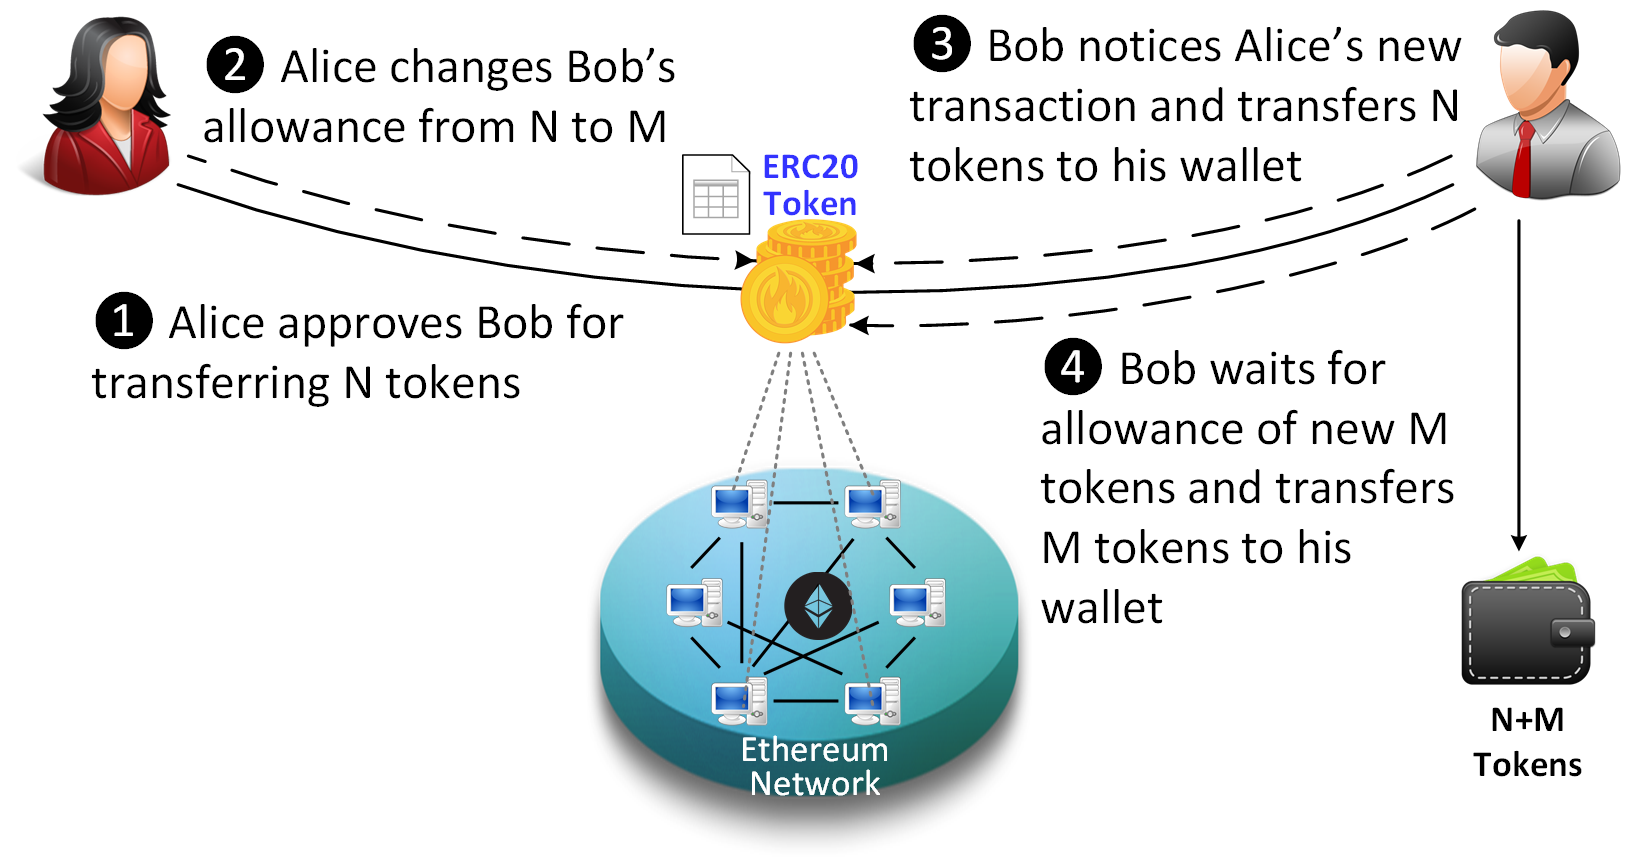
\includegraphics[width=1.0\linewidth]{figures/multiple_withdrawal_02.png}
	\caption{Possible multiple withdrawal attack in ERC20 tokens when Alice changes Bob's allowance from N to M. By front-running, Bob is able to move N+M tokens from Alice's token pool.}
\end{figure}

\subsection{How to prevent the attack}
Sustainable solutions have to prevent Bob from multiple withdrawal (N+M) presuming that Alice has more than N+M tokens in her wallet. One of these approaches can be implemented to prevent the attack:\newline

\begin{enumerate}[label=\Alph*.]
	\item \textbf{Prevention by owner:} This approach is recommended by ERC20 standard \cite{Ref08} and advises owners to change spender allowance from N to 0 and then from 0 to M (instead of set it directly from N to M). Changing allowance to non-zero values after setting to zero will not prevent the attack since the owner would not be able to distinguish how the allowance is set to zero. Was it because of her previous \textit{approve} transaction for changing allowance from N to 0?, Or it was set to 0 by \textit{transferFrom} method due to token transfers? Although It would be possible to track transferred token through \textit{Transfer} events---logged by \textit{transferFrom} method---tracking of tokens would not be easy in case of transferring to a third-party. For example, if Alice allows Bob and then Bob transfers tokens to Carole, \textit{Transfer} event creates a log showing Carole moved tokens from Alice. As discussed in "MiniMeToken" solution, this approach can not prevent the attack despite being recommended by the standard.
	
	\item \textbf{Prevention by \textit{approve} method:} In this approach, \textit{approve} method changes spender allowance from N to M atomically by using compare and set (CAS) pattern \cite{Ref06}. Comparison part of CAS requires knowledge of transferred tokens that reveals any transferred tokens in case of front-running. Hence, we can compare new allowance with transferred token and set it accordingly. Setting new allowance in \textit{approve} method must satisfy ERC20 constraint that says "If this function is called again it overwrites the current allowance with \textit{\_value}" \cite{Ref08}. This constraint prohibits any adjustments in allowance which makes the \textit{approve} method vulnerable. For example, considering front-running by Bob when Alice wants to change Bob allowance form 100 to 110, the \textit{approve} method can reveal 100 transferred tokens by Bob. However, based on ERC20 constraints, it must not adjust new allowance to 110-100=10, it has to set it to 110, which is allowing Bob for transferring 100+110=210 tokens in total. We implemented this approach in proposal 1 and as analyzed, securing \textit{approve} method can not prevent the attack while adhering constraints of the standard. The only feasible approach would be prevention it when transferring tokens.
	
	\item \textbf{Prevention by \textit{transferFrom} method:} This approach is based on ERC20 constraint that says "approve functions allows \textit{\_spender} to withdraw from your account multiple times, up to the \textit{\_value}". So, spender must not be able to transfer more than authorized tokens. That being said, \textit{transferFrom} method can be secured in a way that prevents M new token transfer in case of already transferred N tokens. By comparing transferred tokens in \textit{transferFrom} method, spender will be restricted for moving solely remained tokens. In case of trying to transfer token more than allowed, the transaction fails. For example, Alice's new transaction for increasing Bob allowance from 100 to 110, sets Bob allowance to 110. However, \textit{transferFrom} method does not allow Bob from transferring more than 10 tokens. We implanted this approach in proposal 2 and it prevents the attack effectively.
\end{enumerate}

\subsection{What are violation constraints}
An important criterion for a solution is to adhere the specifications of ERC20 standard. Conforming with the standard, keeps new tokens backward compatible with already deployed smart contracts. So, smart contracts can interact with tokens as defined in the standard without raising any exception. We extracted defined constraints from ERC20 specifications \cite{Ref08} that must be satisfied by any sustainable solution:
\begin{enumerate}
	\item Calling \textit{approve} function has to overwrite current allowance with new allowance.
	\item \textit{approve} method does not adjust allowance, it sets new value of allowance.
	\item Transferring 0 values by \textit{transferFrom} method MUST be treated as normal transfers and fire the \textit{Transfer} event as non-zero transactions.
	\item Introducing new methods violates ERC20 API and it has to be avoided for having compatible token with already deployed smart contracts.
	\item Spender will be allowed to withdraw from approver account multiple times, up to the allowed amount.
	\item Transferring initial allowed tokens is considered as legitimate transfer. It could happen right after approval or before changing allowance.
	\item Race condition MUST not happen in any cases to prevent multiple withdrawal attack account.\newline
\end{enumerate}
% !TEX root = ../main.tex

\newpage
\section{Related work}
Several solutions have been proposed by Ethereum community---mostly from developers on GitHub\cite{Ref07}---to address the attack. There would be some trad-offs for each solution that needs to be evaluated in term of conforming with standard constraints and attack mitigation. We have examined mitigation approach of each solution and explained possible ERC20 constraint violation.

\subsection{Enforcement by User Interface (UI)}
ERC20 standard recommends to set allowance to zero before any non-zero values and enforce approval processing check in UI instead of smart contract:
\begin{figure}[t!]
	\centering
	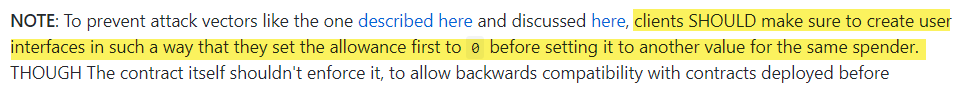
\includegraphics[width=1.0\linewidth]{figures/multiple_withdrawal_03.png}
	\caption{Recommendation of ERC20 standard to mitigate multiple withdrawal attack by enforcement in UI.}
\end{figure}


\noindent If Alice does not use UI and connects directly to the blockchain, there would be a good chance of impacting by this attack. Even if she uses UI, this approach can not prevent the attack. As discussed on GitHub\cite{Ref14}, Bob still can transfer N+M tokens in the below scenario:
\begin{enumerate}
	\item Bob is allowed to transfer N Alice’s tokens.
	\item Alice publishes a new transaction that changes Bob’s allowance from N to 0.
	\item Bob front runs Alice’s transaction and transfers N Alice’s tokens (\textit{transferFrom} sets Bob’s allowance to 0 respectively).
	\item Alice’s transaction is mined and sets Bob’s allowance to 0.
	\item Now Alice publishes a new transaction that changes Bob’s allowance from 0 to M.
	\item Alice’s second transaction is mined, Bob now is allowed to move M Alice’s tokens.
	\item Bob transfers M Alice’s tokens and in total N+M.\newline
\end{enumerate}
At step 3, Bob is able to transfer N tokens and consequently his allowance becomes 0 by \textit{transferFrom} method. This is considered as a legitimate transaction since Alice has already approved it. The issue occurs after Alice’s new transaction in step 5 to set Bob's allowance to M. In case of front-running by Bob, Alice needs to check Bob’s allowance for the second time before setting any new value. However, she finds out Bob’s allowance 0 in either case. In other words, she can not distinguish whether Bob’s allowance is set to 0 because of her transaction in step 2 or Bob already transferred tokens by front-running is step 3 and that made his allowance 0. Someone may point out that Alice notices this by checking \textit{Transfer} event logged by \textit{transferFrom} function. However, if Bob had transferred tokens to someone else (like Carol), then \textit{Transfer} event will not be linked to Bob, and, if Alice’s account is busy and many people are allowed to transfer from it, Alice may not be able to distinguish this transfer from a legitimate one performed by someone else. Overall, this solution does not prevent the attack while tries to follow ERC20 recommendations for setting Bob’s allowance to zero before any non-zero value. Hence, enforcement should be considered at contract level not UI to remove the gap between transactions and mitigate the attack. Interestingly, OpenZeppelin example implements a workaround in contract level that makes it inconsistent with the recommendations of ERC20. 

\subsection{Minimum viable token}
As suggested by Ethereum Foundation\cite{Ref05}, we can boil down ERC20 standard to a very basic functionalities by implementing only essential methods. this will prevent effecting of the attack by skipping implementation of vulnerable functions. While removing \textit{approve} and \textit{transferFrom} functions prevent the attack, it makes the token partially-ERC20-compliant. Golem Network Token (GNT\footnote{https://etherscan.io/address/0xa74476443119A942dE498590Fe1f2454d7\newline D4aC0d\#code}) is one of these examples since it does not implement the \textit{approve}, \textit{allowance} and \textit{transferFrom} functions. According to ERC20 specifications\cite{Ref08}, these methods are not OPTIONAL and must be implemented. Moreover, ignoring them will cause failed function calls from standard smart contracts that expect to interact with these methods. Therefore, we would not consider it as backward compatible solution although mitigates the attack by removing vulnerable functions.

\subsection{Approving trusted parties}
Approving token transfer to non-upgradable smart contracts can be considered safe. Because they do not contain any logic to take advantage of this vulnerability. However, upgradable smart contracts may add new logic to new versions that needs code re-verification before approving token transfers. Similarly, approving token transfer to people that we trust could be considered as a mitigation plan. Nonetheless, this solution would have limited use cases and it could not be considered as a comprehensive mitigation for the attack.

\subsection{MiniMeToken}
MiniMeToken\cite{Ref15} followed ERC20 recommendation by setting allowance to zero before non-zero values. They added a line of code to their \textit{approve} method. The red clause (\textit{\_amount == 0}) allows setting of approval to 0 and blue condition checks allowance of \textit{\_spender} to be 0 before setting to non-zero values (i.e., If \textit{\_spender} allowance is 0 then allows non-zero values):
\begin{figure}[t]
	\centering
	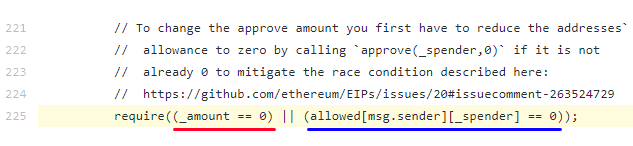
\includegraphics[width=1.0\linewidth]{figures/multiple_withdrawal_06.png}
	\caption{MiniMeToken added code to \textit{approve} method for allowing non-zero allowance values if it is already set to zero.}
\end{figure}
\noindent Similar to "Enforcement by User Interface (UI)", this will not prevent Bob from transferring N+M tokens. Because Alice would not be able to distinguish whether N tokens have been already transferred or not. It is more clear in the below scenario:
\begin{enumerate}
	\item Alice decides to set Bob’s allowance to 0.
	\item Bob front-runs Alice’s transaction and his allowance sets to 0 after transferring N tokens.
	\item Alice’s transaction is executed and sets Bob’s allowance to 0 (Red clause passes sanity check).
	\item Alice checks Bob’s allowance and she will find it 0, so, she can not determine whether this was because of her transaction or Bob already transferred N tokens.
	\item Alice considers that Bob has not been transferred any tokens and allows him for transferring new M tokens.
	\item Bob is able to transfer new M tokens and N+M in total.
\end{enumerate}

\subsection{MonolithDAO}
MonolithDAO Token\cite{Ref12} implements two additional functions for allowance increase or decrease. The default \textit{approve} function has additional codes to enforce owner for setting allowance to zero before non-zero values. It allows non-zero spender's allowance if it is already set to zero. The below table shows functionality of \textit{approve} method based on current spender's allowance and passed input \textit{\_value} as new allowance:
\begin{figure}[t]
	\centering
	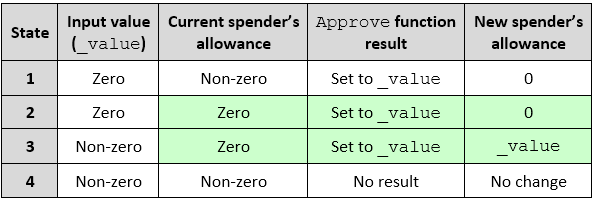
\includegraphics[width=1.0\linewidth]{figures/multiple_withdrawal_09.png}
	\caption{Functionality of default \textit{approve} method in MonolithDAO token that enforces setting spender's allowance to zero before any non-zero values. It implements ERC20 recommendation for changes allowance from N to M in two steps (N$\rightarrow$0$\rightarrow$M).}
\end{figure}
\noindent If the current spender’s allowance is non-zero, \textit{decreaseApproval}\footnote{decreaseApproval(address \textit{\_spender}, uint \textit{\_subtractedValue})} and \textit{increaseApproval}\footnote{increaseApproval(address \textit{\_spender}, uint \textit{\_addedValue})} functions have to be used for decreasing or increasing the allowance. Using these two functions can prevent race condition and mitigate the attack as explained below:
\begin{enumerate}
	\item Alice allows Bob to transfer N tokens by calling \textit{approve(\_Bob, N)}. Alice used the default \textit{approve} function consciously since current Bob’s allowance is 0. So, he checked Bob's allowance before calling \textit{approve} method.
	\item After a while, Alice decides to decrease Bob’s approval by M and runs \textit{decreaseApproval(\_Bob, M)}.
	\item Bob notices Alice’s second transaction and front runs it by executing \textit{transferFrom(\_Alice, \_Bob, N)}.
	\item Bob’s transaction will be executed first and transfers N token to his account and the his allowance becomes 0 as result of this transfer.
	\item Alice’s transaction is mined after Bob’s transaction and tries to decrease Bob’s allowance by M. If Bob had already transferred more than M tokens, new Bob’s allowance becomes negative and it fails the transaction. So, the transaction does not change Bob’s remaining allowance and he would be able to transfer the rest (which is legitimate transfer since Alice has already approved it). If Bob had transferred less than M tokens, the new allowance will be applied and reduces Bob’s allowance by M.\newline
\end{enumerate}
\noindent Although these two new functions will prevent the attack, they have not been defined in the initial specifications of ERC20. Therefore, they can not be used by smart contracts that are already deployed on the Ethereum network and still call approve method for setting new allowance---and not \textit{increaseApproval} or \textit{decreaseApproval}. Moreover, ERC20 specifications does not define any increase or decrease of allowance. It only allows setting new allowances without adjustment. For example, if Alice has approved Bob for 100 tokens and wants to set it to 80, the new allowance should be 80 while using decrease methods will set it 20 (100 - 80 = 20). Comparatively, increase method will set new allowance to 180 while it has to set it to 80 again to be in-compliant with ERC20 specification. For these reasons, this solution would not be compatible with ERC20 standard and only is usable if approver or smart contract are aware of these supplementary methods.

\subsection{Alternate approval function}
Another suggestion\cite{Ref16} is to move security checks to another function called \textit{safeApprove}\footnote{safeApprove(address \textit{\_spender}, uint256 \textit{\_currentValue}, uint256 \textit{\_value})} that compare current and new allowance values and sets it if has not been already changed. By using this function, Alice uses the standard \textit{approve} function to set Bob’s allowance to 0 and for new approvals, she has to use \textit{safeApprove} function. \textit{safeApprove} takes the current expected approval amount as input parameter and calls \textit{approve} method if previous allowance is equal to the current expected approval. By using this function, Alice will have one step more to read the current allowance and pass it to the new \textit{safeApprove} method. Although this approach mitigates the attack by using CAS pattern\cite{Ref06}, however, it is not backward compatible with already implemented smart contracts due to their unawareness of this new complementary function. In other words, the new \textit{safeApprove} method is not defined in ERC20 standard and existing smart contracts would not be able to use this new safety feature.

\subsection{Detecting token transfers}
In order to set new allowance atomically, tracking of transferred tokens is required to detect token transfers before setting new allowances. If \textit{approve} method reveals any transferred tokens due to front running, it throws an exception without setting new allowance. As suggested by \cite{Ref17}, a flag can be used to detect whether any tokens have been transferred or not. \textit{transferFrom} method sets this flag to \textit{true} in case of any token transfer. \textit{approve} method checks the flag to be \textit{false} before allowing new approvals. This approach requires new data structure to keep track of used/transferred tokens for each spender. It can prevent race condition as described below:
\begin{enumerate}
	\item Alice runs \textit{approve(\_Bob, N)} to allow Bob for transferring N tokens. Since Bob’s initial allowance is 0 and his corresponding flag=\textit{false}, then sanity check passes and Bob’s allowance sets to N in line 15.
	\item Alice decides to set Bob’s allowance to 0 by executing \textit{approve(\_Bob, 0)}.
	\item Bob front-runs Alice’s transaction and transfers N tokens. Then, \textit{transferFrom} turns his flag to \textit{true}.
	\item Alice’s transaction is mined and passes sanity check because passed value is 0.
	\item Bob’s allowance is set to 0 while his flag remains \textit{true}. (\textit{approve} method does not flip spender flags.)
	\item Alice wants to change Bob’s allowance to M by executing \textit{approve(\_Bob, M)}. Since Bob already transferred N tokens (his flag=\textit{true}), the transaction fails.
	\item Bob’s allowance does not change and he cannot move more tokens than initially allowed.\newline
\end{enumerate}
\noindent Although this approach mitigates the attack, it prevents any further legitimate approvals as well. Considering a scenario that Alice rightfully wants to increase Bob’s allowance from N to M (two non-zero values). If Bob had already transferred number of tokens, Alice would not be able to change his approval. Because Bob's flag is set to \textit{true} and line 15 does not allow changing allowance by throwing an exception:
\begin{figure}[t]
	\centering
	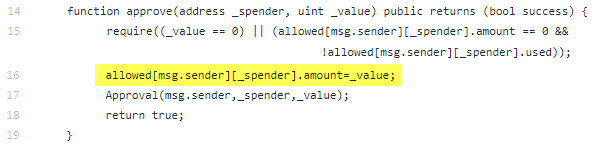
\includegraphics[width=1.0\linewidth]{figures/multiple_withdrawal_33.png}
	\caption{\textit{approve} method needs to be modifed by adding a line of code like \textit{allowed[msg.sender][\_spender].used = false;} between lines 16 and 17 to unlock spender flag for the next legitimate change.}
\end{figure}
\noindent Even setting allowance to 0 and then to M, does not flip the flag to \textit{false} (There is no code for it in the \textit{approve} method). So, It keeps Bob’s allowance locked down and blocked further legitimate allowances. In fact, \textit{approve} method needs a new code between lines 16 and 17 to set the flag to \textit{false}. But it will cause another problem. After setting allowance to 0, spender flag becomes \textit{false} and allows non-zero values event if tokens have been already transferred. It resembles the initial state of allowance similar when nothing was transferred. For example, considering front-running by Bob, before new allowance change from N to 0 by Alice. Bob's flag turns to \textit{true} by \textit{transferFrom} method and turns to \textit{false} by \textit{approve} method afterwards. Now if Alice wants to set allowance from 0 to M, Bob's flag is \textit{false} and his allowance is zero. This is similar to the situation that he did not transfer any tokens. So, Alice cannot distinguish whether Bob moved any token or not. Setting new allowance will allow Bob to transfer more tokens than Alice wanted. Therefore, adding new code makes attack mitigation functionality ineffective. In short, this approach can not satisfy both legitimate and non-legitimate scenarios. Nevertheless, it is a step forward by introducing the need for a new variable to track transferred tokens.

\subsection{Keeping track of remaining tokens}
This approach\cite{Ref18} is inspired by the previous solution and keeping track of remaining tokens instead of detecting transferred tokens. It uses modified version of data structure that used in the previous solution for storing residual tokens:
\begin{figure}[t]
	\centering
	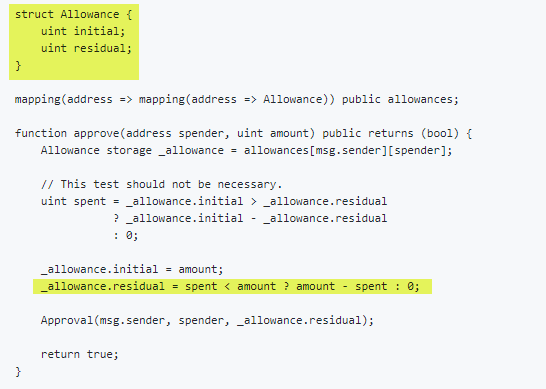
\includegraphics[width=0.9\linewidth]{figures/multiple_withdrawal_29.png}
	\caption{Keeping track of remaining tokens.}
\end{figure}
\noindent At first, it seems to be a promising solution by setting approval to zero before non-zero values. However, the highlighted code in \textit{approve} method resembles the situation that we explained in "Enforcement by User Interface (UI)". It would not be possible for Alice to distinguish if any token transfer have occurred when changing allowance. To make it more clear, considering the below scenario:  
\begin{enumerate}
	\item Bob’s allowance is initially zero (\textit{allowances[\_Alice][\_Bob].initial=0}) and his residual is zero as well (\textit{allowances[\_Alice][\_Bob].residual=0}).
	\item Alice allows Bob to transfer N tokens that makes \textit{allowances[\_Alice][\_Bob].initial=N} and \textit{allowances[\_Alice][\_Bob].residual=N}.
	\item Alice decides to change Bob’s allowance to M and has to set it to zero before any non-zero values.
	\item Bob noticed Alice’s transaction for setting his allowance to zero and transfers N tokens in advance. Consequently, \textit{transferFrom} function sets his residual to zero (\textit{allowances[\_Alice][\_Bob].residual=0}).
	\item Alice’s transaction for setting Bob's allowance to zero is mined and sets \textit{allowances[\_Alice][\_Bob].initial=0} and \textit{allowances[\_Alice][\_Bob].residual=0} This is similar to step 1 that no token has been transferred. So, Alice would not be able to distinguish whether any token have been transferred or not.
	\item Considering no token transfer by Bob, Alice approves Bob for spending new M tokens.
	\item Bob is able to transfer new M tokes in addition to initial N tokens.\newline
\end{enumerate}
Someone may think of using \textit{Transfer} event to detect transferred tokens or checking approver balance to see any transferred tokens. As explained in "Enforcement by User Interface (UI)", using \textit{Transfer} event is not sufficient in case of transferring tokens to a third party. Checking approver balance also would not be an accurate way if the contract is busy and there are lot of transfers. So, it would be difficult for the approver to detect legitimate from non-legitimate tokens transfers. Overall, this approach cannot prevent the attack.

\subsection{Changing ERC20 API}
As advised by \cite{Ref03}, changing ERC20 API could secure \textit{approve} method by comparing current allowance of the spender and sets it to new value if it has not already been transferred any tokens. This allows atomic compare and set of spender allowance to make the attack impossible. So, it will need new overloaded \textit{approve} method with three parameters in addition to the standard \textit{approve} method with two parameters:
\begin{figure}[t]
	\centering
	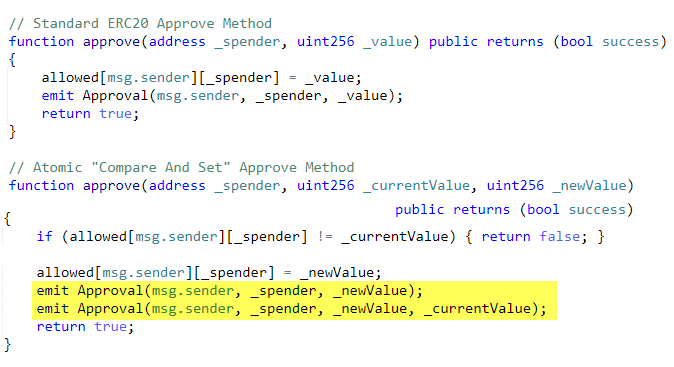
\includegraphics[width=1.0\linewidth]{figures/multiple_withdrawal_12.png}
	\caption{Suggested ERC20 API Change by adding new \textit{approve} method with three parameters to compare and set new allowance atomically.}
\end{figure}
\noindent In order to use this new method, smart contracts have to update their codes to provide three parameters instead of current two, otherwise any \textit{approve} call will use the standard vulnerable version. Moreover, one more call is required to read current allowance and pass it to the new \textit{approve} method. New event definition needs to be added to ERC20 API to log an approval events with four arguments. For backward compatibility reasons, both three-arguments and new four-arguments events have to be logged. All of these changes makes this token contract incompatible with already deployed smart contracts.

\subsection{New token standards}
After recognition of this security vulnerability, new standards like ERC233 \footnote{https://github.com/Dexaran/ERC223-token-standard}, ERC721\footnote{https://github.com/ethereum/EIPs/blob/master/EIPS/eip-721.md} and ERC777\footnote{https://eips.ethereum.org/EIPS/eip-777} were introduced to address the issue in addition to improving current functionality of ERC20 standard. They changed approval model and fixed some drawbacks which need to be addressed in ERC20 as well (i.e., handle incoming transactions through a receiver contract, lost of funds in case of calling \textit{transfer} function instead of \textit{transferFrom}, etc). Nevertheless, migration from ERC20 to ERC223/ERC721/ERC777 would not be convenient and all deployed ERC20 tokens (168,092\footnote{https://etherscan.io/tokens} tokens as of 18 February 2019) needs to be redeployed. This also means update of any trading platform listing ERC20 tokens. The goal here is to find a backward compatible solution instead of changing current ERC20 standard or migrating tokens to a new standards. Despite expanded features and improved security properties of new standards, we would not consider them as target solutions.
% !TEX root = ../main.tex

\section{Proposals}
\subsection{Proposal 1: Securing \textit{approve} method}
As discussed in the previous section, a sustainable solution should use CAS pattern\cite{Ref06} to set new allowance atomically. This needs knowledge of transferred tokens that requires adding a new mapping variable to the token code. The code is still compatible with other smart contracts due to internal usage of the variable. Modified version of \textit{transferFrom} method can track transferred tokens by storing them in this new variable (\textit{transferred}):
\begin{figure}[t]
	\centering
	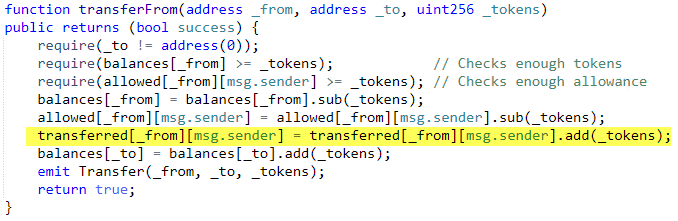
\includegraphics[width=1.0\linewidth]{figures/multiple_withdrawal_14.png}
	\caption{Modified version of \textit{transferFrom} for keeping track of transferred tokens per spender.}
\end{figure}
\noindent Similarly, a block of code is added to the \textit{approve} function to work in both cases with zero and non-zero allowances. Added code compares new allowance (passed as \textit{\_tokens} to the function) with the current allowance of the spender and already transferred token (highlighted as \textit{allowed[msg.sender][\_spender]} and \textit{transferred[msg.sender][\_spender]} respectively). Then it decides to increase or decrease current allowance based on this comparison. If the new allowance is less than initial allowance (sum of \textit{allowance} and \textit{transferred} variables), it denotes decreasing allowance, otherwise increasing allowance was intended.
\begin{figure}[t]
	\centering
	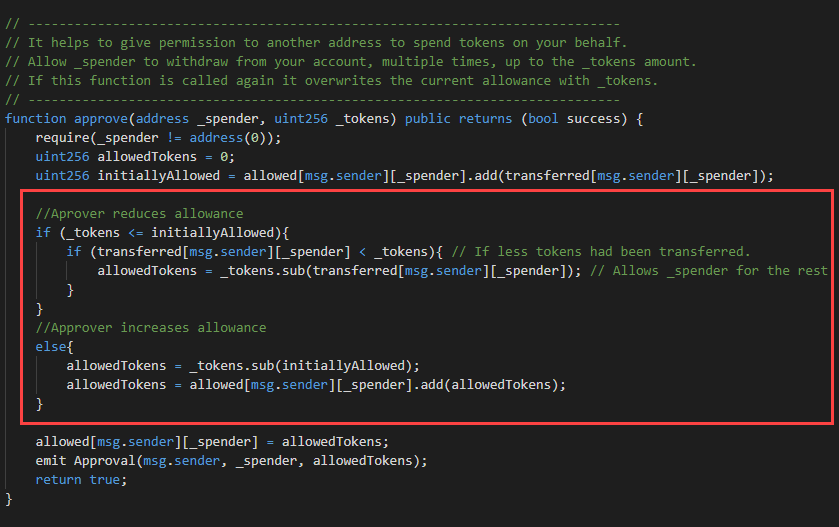
\includegraphics[width=1.0\linewidth]{figures/multiple_withdrawal_15.png}
	\caption{Added code block to \textit{approve} function to prevent the attack by comparing and setting new allowance atomically.}
\end{figure}
\noindent Modified \textit{approve} function prevents the attack in either increasing or decreasing of the allowance. Unlike other solutions, there is no need to set allowance from N to 0 and then to M. The owner can directly change the allowance from N to M which is saving one transaction accordingly. Considering the below scenarios when decreasing or increasing allowance:\newline\newline
\noindent \textbf{A.} Alice approves Bob for spending 100 tokens and then decides to decrease it to 10 tokens.
\begin{enumerate}
	\item Alice approves Bob for transferring 100 tokens.
	\item After a while, Alice decides to reduce Bob’s allowance from 100 to 10 tokens.
	\item Bob noticed Alice’s new transaction and transfers 100 tokens by front-running.
	\item Bob’s allowance is 0 and \textit{transferred} is 100 (set by \textit{transferFrom} function).
	\item Alice’s transaction is mined and checks initial allowance (100) with new allowance (10).
	\item As it is reducing, \textit{transferred} tokens (100) is compared with new allowance (10). Since Bob already transferred more tokens, his allowance will be set to 0.
	\item Bob is not able to move more than initial 100 approved tokens.\newline
\end{enumerate}

\noindent \textbf{B.} Alice approves Bob for spending 100 tokens and then decides to increase it to 120 tokens.
\begin{enumerate}
	\item Alice approves Bob for transferring 100 tokens.
	\item After a while, Alice decides to increase Bob’s allowance from 100 to 120 tokens.
	\item Bob noticed Alice’s new transaction and transfers 100 tokens by front-running.
	\item Bob’s allowance is 0 and \textit{transferred} is 100.
	\item Alice’s transaction is mined and checks initial allowance (100) with new allowance (120).
	\item As it is increasing, new allowance (120) will be subtracted from transferred tokens (100).
	\item 20 tokens will be added to Bob’s allowance.
	\item Bob would be able to transfer more 20 tokens (120 in total as Alice wanted).\newline
\end{enumerate}
\noindent In order to evaluate functionality of the new \textit{approve}/\textit{transferFrom} functions, we have implemented a standard ERC20 token (TKNv1\footnote{https://rinkeby.etherscan.io/address/0x8825bac68a3f6939c296a40fc8078\newline d18c2f66ac7}) along side proposed ERC20 token (TKNv2\footnote{https://rinkeby.etherscan.io/address/0xf2b34125223ee54dff48f71567d4b\newline 2a4a0c9858b}) on Rinkeby test network. Result of tests for different input values shows that TKNv2 can address multiple withdrawal attack by making front-running gain ineffective. Moreover, we compared these two tokens in term of gas consumption. TokenV2.\textit{approve} function uses almost the same amount of gas as TokenV1.\textit{approve}, however, gas consumption of TokenV2.\textit{transferFrom} is around 47\% more than TokenV1.\textit{transferFrom}. This difference is because of maintaining a new mapping variable for tracking transferred tokens:
\begin{figure}[t]
	\centering
	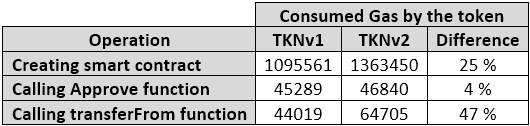
\includegraphics[width=1.0\linewidth]{figures/multiple_withdrawal_22.png}
	\caption{Comparison of gas consumption between standard implementation of ERC20 token (TKNv1) and secured implemetation (TKNv2).}
\end{figure}
\noindent In term of compatibly, working with standard wallets (like MetaMask) have not raised any transfer issue. This shows compatibility of the token with existing wallets. In summary, we could use CAS pattern to implement a secure \textit{approve} method that can mitigate the attack effectively. However, it violates one of ERC20 specifications that says "If this function is called again it overwrites the current allowance with \textit{\_value}". This implementation of \textit{approve} method adjusts allowance based on transferred tokens. Essentially, it would not be possible to secure the \textit{approve} method without adjusting the allowance. Considering the below scenario:
\begin{enumerate}
	\item Alice decides to change Bob's allowance from N to M (M<N in this example).
	\item Bob transfers N tokens by front running and \textit{transferred} variable sets to N.
	\item Alice's transaction is mined and \textit{approve} method detects token decrease. If \textit{approve} method does not adjust the allowance based on transferred tokens, it has to set it to M (to conform the standard) which is allowing Bob to transfer more M tokens.
\end{enumerate}
Therefore, \textit{approve} method has to adjust the allowance according to transferred tokens, not based on passed input values. Overall, there is no solution to secure \textit{approve} method while adhering specification of ERC20 standard.

\subsection{Proposal 2: Securing \textit{transferFrom} method}
As an alternative solution, we can think of securing \textit{transferFrom} method instead of \textit{approve} function. the goal here is to prevent spender from transferring more tokens than allowed. Based on this assumption, we should not consider allowance as the main factor. Transferred tokens can be considered as the main variable in calculations. For example in the below situation we can prevent the attack by securing \textit{transferFrom} method and keeping \textit{approve} function as default:
\begin{enumerate}
	\item Alice allowed Bob for transferring 100 tokens and decides to set it to 70 after a while.
	\item Bob front runs Alice’s transaction and transfers 100 tokes (legitimate transfer).
	\item Alice’s transaction is mined and sets Bob allowance to 70 by the default \textit{approve} method.
	\item Bob noticed new allowance and tries to move new tokens by running \textit{transferFrom(\_Bob,70)}. Since he already transferred more than 70, his transaction fails and prevents multiple withdrawal. Additionally, Bob’s allowance stays as 70, although transferred tokens shows 100.
\end{enumerate}
Here allowance can be considered as maximum allowance. It indicates that Bob is eligible to transfer up to specified limit if he has not already transferred any tokens. This impression is completely in accordance with ERC20 standard that emphasizes:
\begin{figure}[t]
	\centering
	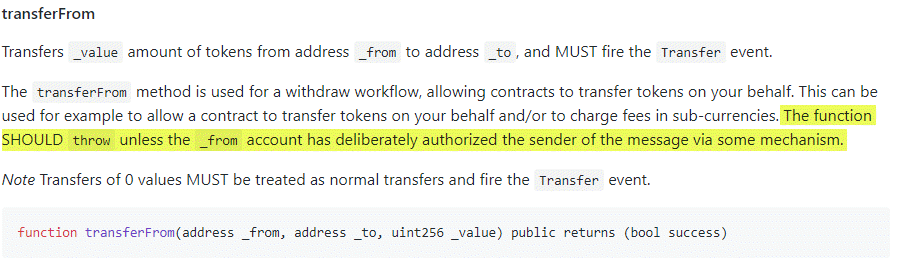
\includegraphics[width=1.0\linewidth]{figures/multiple_withdrawal_30.png}
	\caption{ERC20 \textit{transferFrom} method that emphasizes on throwing exception if spender is not authorized to move tokens.}
\end{figure}
\noindent By this assumption, we secured \textit{transferFrom} method instead of \textit{approve} method by adding required codes to prevent more token transfer that allowed:
\begin{figure}[t]
	\centering
	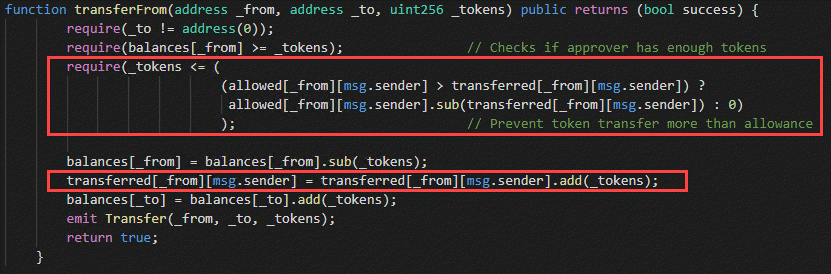
\includegraphics[width=1.0\linewidth]{figures/multiple_withdrawal_31.png}
	\caption{Securing \textit{transferFrom} method instead of \textit{approve} method.}
\end{figure}
\noindent In fact, there is no relation between allowance (\textit{allowed[\_from][msg.sender]}) and transferred tokens (\textit{transferred[\_from][msg.sender]}). The fist variable shows maximum transferable tokens by a spender and can be changed irrelative to transferred tokens (i.e., \textit{approve} method does not check transferred tokens). If Bob has not already transferred that much of tokens, he would be able to transfer difference of it \textit{allowed[\_from][msg.sender].sub(transferred[\_from][msg. sender]}). In other words, transferred is life time variable that accumulates transferred tokens regardless of allowance change. This token is implemented as TKNv3\footnote{https://rinkeby.etherscan.io/address/0x5d148c948c01e1a61e280c8b2ac39\newline fd49ee6d9c6} on Rinkby network and passed compatibility by transferring tokens. In terms of gas consumption, \textit{transferFrom} function needs at about 37\% more gas than standard \textit{transferFrom} implementation which is acceptable for having a secure ERC20 token.
% !TEX root = ../main.tex

\section{Conclusion}

The development of smart contracts has proven to be error-prone in practice, and as a result, contracts deployed on public platforms are often riddled with security vulnerabilities. Exploited by the attackers, these vulnerabilities can often lead to major security incidents which introduce great cost due to the immutability characteristics of the blockchain technology. In this paper, we examine \erc security vulnerabilities and thoroughly discuss the technical details, the circumstances of the incidents together with their impacts and mitigations. We also integrate best practices to improve efficiency and productivity of the token. Eventually, we propose a secure \erc code that is not vulnerable to any of the attacks. Using auditing tools and comparing with the top ten \erc tokens shows the security of the proposal. It can be used as template to deploy new \erc tokens, migrate current vulnerable deployments or develop tools to automate auditing of \erc tokens.

{\chg Highlights for inducing in the conclusion:
\begin{itemize}
	\item At about 98\% of tokens are \erc, showing importance of security
	\item There is no vulnerability reference site (like https://swcregistry.io) for \erc tokes. We collected them all in the paper.
	\item Some vulnerabilities are specific to \erc token that cannot be categorized under smart contract vulnerabilities, so, need separate work as we did
	\item We provided list of \num vulnerabilities for \erc tokens by including best practices to improve the performance and make it ready for industrial implementations (\eg ICOs, DApps, \etc)
	\item \sys passed all audits of 7 tools, proving its security against current Ethereum vulnerabilities. Also, detected security issue in the comparison table are false positives that are considered as failed check for \sys to make a fair comparison
	\item The code is available in compatible Solidity version (0.5.11) and the recent versions (0.7.2), but the recent one may not be used by audit tools.
	\item We ignored some known tools (like Oyente) due to their support from legacy Solidity versions (knows compiler bugs).
	\item If businesses are looking for a secure token, \sys can be used as a template and customized with advanced features (like multi parties approval for withdrawing ETH).
\end{itemize}

}




%=====================================================================================
\bibliographystyle{abbrv}
\footnotesize
\bibliography{references}
\end{document}
%=====================================================================================